
% This LaTeX was auto-generated from MATLAB code.
% To make changes, update the MATLAB code and republish this document.

\documentclass{article}
\usepackage{graphicx}
\usepackage{color}

\sloppy
\definecolor{lightgray}{gray}{0.5}
\setlength{\parindent}{0pt}

\begin{document}

    
    
\subsection*{Contents}

\begin{itemize}
\setlength{\itemsep}{-1ex}
   \item Rocket Problem
   \item Clearing console and variables.
   \item Declaring constant values given from problem statement.
   \item Intermediate calculations of various values.
   \item No atmosphere, no pitchover angle.
   \item No atmosphere, 0.1 rad pitchover angle.
   \item Atmosphere, 0.1 rad pitchover angle.
   \item Atmosphere, 0.1 rad pitchover angle, changing parameters
   \item Rates function called by ODE45.
\end{itemize}


\subsection*{Rocket Problem}

\begin{par}
Spaceflight Mechanics - Spring 2019 Johnathan Corbin
\end{par} \vspace{1em}
\begin{verbatim}
function RocketProblem
\end{verbatim}


\subsection*{Clearing console and variables.}

\begin{verbatim}
clear, clc
\end{verbatim}


\subsection*{Declaring constant values given from problem statement.}

\begin{verbatim}
Isp = 353; %LOx - Kerosene propellant, [s]
epsilon = 0.01; %Rocket's structural ratio
mass_L = 1000; %Payload mass, [kg]
mass_P = 10000; %Propellant mass, [kg]
diameter = 1.65; %Rocket diameter, [m]
t_burn = 240; %Total burn time, [s]
r_earth = 6378 * 1000; %Radius of the Earth, [m]
t0 = 0; %Initial time, [s]
pitch = 500; %Height at which pitchover begins, [m]
u = 398600 * 1000^3; %Standard gravitational parameter for Earth, [m^3/s^2]
s_g = 9.81; %Standard gravity, [m/s^2]
rho0 = 1.225; %Sea level air density, [kg/m^3]
hscale = 7500; %Density scale height, [m]
\end{verbatim}


\subsection*{Intermediate calculations of various values.}

\begin{verbatim}
A = pi * (diameter / 2)^2; %Frontal area of the rocket, [m^2]
tspan = [t0, t_burn]; %Time range for the integrator, [s]
mass_structure = -epsilon * mass_P / (epsilon - 1); %Structural mass of the rocket, [kg]
m_dot = mass_P / t_burn; %Mass rate of ejecta, [kg/s]
thrust = m_dot * Isp * s_g; %Thrust generated by ejecta, [N]
\end{verbatim}


\subsection*{No atmosphere, no pitchover angle.}

\begin{verbatim}
theta0 = 0; %Pitchover angle, [rad]
Cd = 0; %Drag coefficient
v0 = 0; %Initial velocity, [m/s]
x0 = 0; %Initial downrange distance, [m]
h0 = 0; %Initial height, [m]

f0 = [v0, theta0, x0, h0]; % Initial conditions vector
Opt1 = odeset('Events', @Begin_Pitch);
[time, f] = ode45(@rocketMan, tspan, f0, Opt1);
v = f(:, 1);
theta = f(:, 2);
x = f(:, 3);
h = f(:, 4);

figure(1)
plot(x / 1000, h / 1000, '--k')
hold on

v0 = v(end); %Initial velocity, [m/s]
x0 = x(end); %Initial downrange distance, [m]
h0 = h(end); %Initial height, [m]

tspan = [time(end), t_burn];
f0 = [v0, theta0, x0, h0];
Opt2 = odeset('Events', @Crashed);
[~, f] = ode45(@rocketMan2, tspan, f0, Opt2);
v = f(:, 1);
theta = f(:, 2);
x = f(:, 3);
h = f(:, 4);

plot(x / 1000, h / 1000, '--k')
grid on
title('No Atmosphere, No Pitch')
xlabel('Downrange [km]')
ylabel('Height [km]')
\end{verbatim}

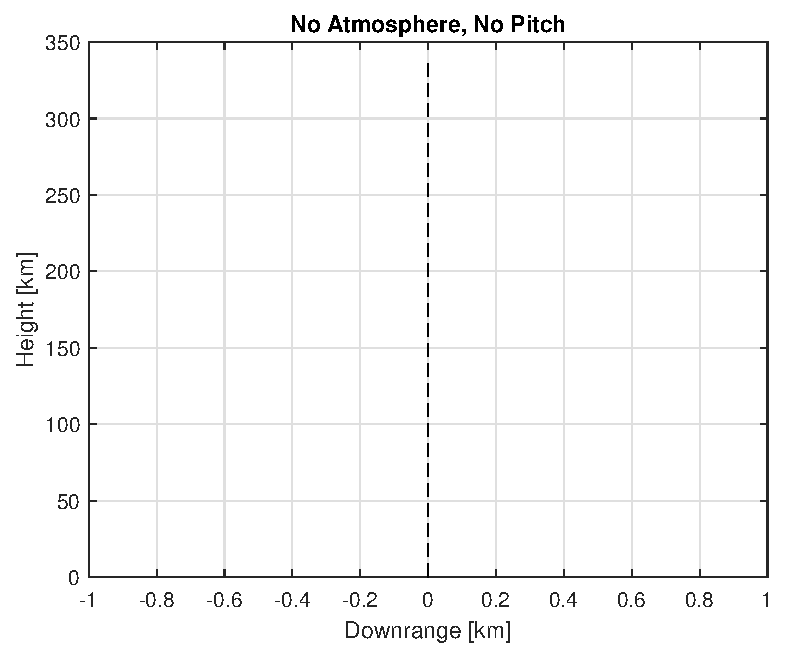
\includegraphics [width=4in]{RocketProblem_01.eps}


\subsection*{No atmosphere, 0.1 rad pitchover angle.}

\begin{verbatim}
theta0 = 0.1 * pi / 180; %Pitchover angle, [rad]
Cd = 0; %Drag coefficient
v0 = 0; %Initial velocity, [m/s]
x0 = 0; %Initial downrange distance, [m]
h0 = 0; %Initial height, [m]
tspan = [t0, t_burn];

f0 = [v0, 0, x0, h0]; % Initial conditions vector
Opt1 = odeset('Events', @Begin_Pitch);
[time, f] = ode45(@rocketMan, tspan, f0, Opt1);
v = f(:, 1);
theta = f(:, 2);
x = f(:, 3);
h = f(:, 4);

figure(2)
plot(x / 1000, h / 1000, '--k')
hold on

v0 = v(end); %Initial velocity, [m/s]
x0 = x(end); %Initial downrange distance, [m]
h0 = h(end); %Initial height, [m]

tspan = [time(end), t_burn];
f0 = [v0, theta0, x0, h0];
Opt2 = odeset('Events', @Crashed);
[~, f] = ode45(@rocketMan2, tspan, f0, Opt2);
v = f(:, 1);
theta = f(:, 2);
x = f(:, 3);
h = f(:, 4);

p(1) = plot(x / 1000, h / 1000, '--k');
grid on
title('0.1 Rad Pitch')
xlabel('Downrange [km]')
ylabel('Height [km]')
\end{verbatim}

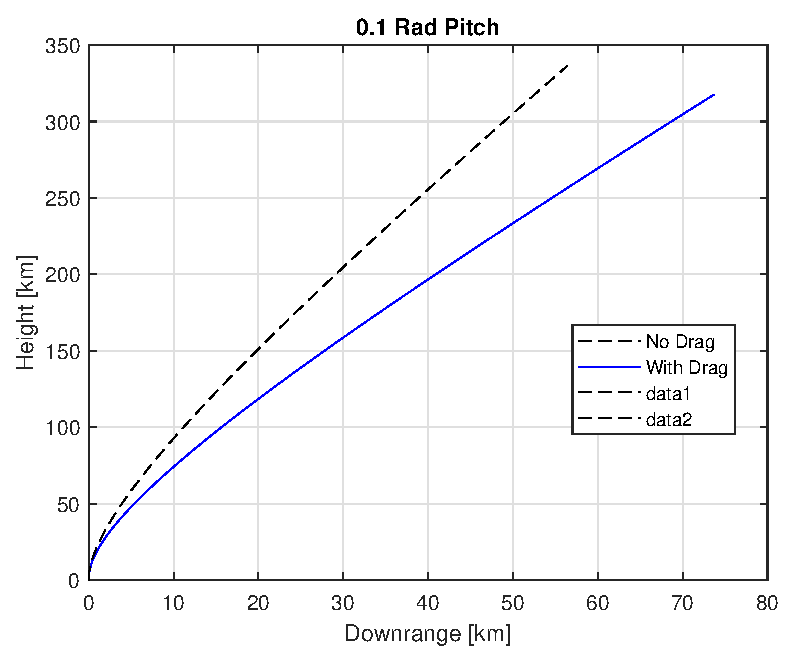
\includegraphics [width=4in]{RocketProblem_02.eps}


\subsection*{Atmosphere, 0.1 rad pitchover angle.}

\begin{verbatim}
theta0 = 0.1 * pi / 180; %Pitchover angle, [rad]
Cd = 0.3; %Drag coefficient
v0 = 0; %Initial velocity, [m/s]
x0 = 0; %Initial downrange distance, [m]
h0 = 0; %Initial height, [m]
tspan = [t0, t_burn];

f0 = [v0, 0, x0, h0]; % Initial conditions vector
Opt1 = odeset('Events', @Begin_Pitch);
[time, f] = ode45(@rocketMan, tspan, f0, Opt1);
v = f(:, 1);
theta = f(:, 2);
x = f(:, 3);
h = f(:, 4);

plot(x / 1000, h / 1000, 'b')
hold on

v0 = v(end); %Initial velocity, [m/s]
x0 = x(end); %Initial downrange distance, [m]
h0 = h(end); %Initial height, [m]

tspan = [time(end), t_burn];
f0 = [v0, theta0, x0, h0];
Opt2 = odeset('Events', @Crashed);
[~, f] = ode45(@rocketMan2, tspan, f0, Opt2);
v = f(:, 1);
theta = f(:, 2);
x = f(:, 3);
h = f(:, 4);

p(2) = plot(x / 1000, h / 1000, 'b');
legend(p([1 2]), 'No Drag','With Drag', 'location', 'best')
\end{verbatim}

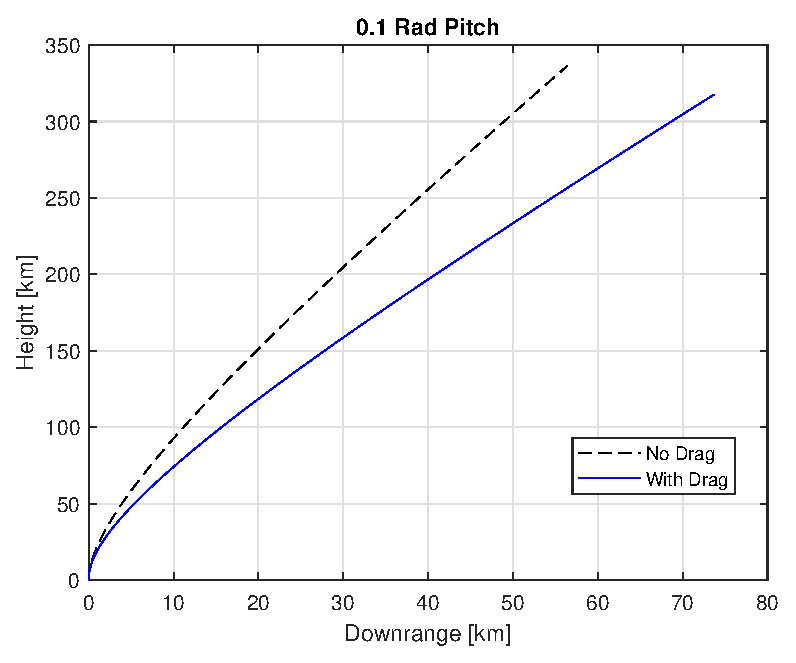
\includegraphics [width=4in]{RocketProblem_03.eps}


\subsection*{Atmosphere, 0.1 rad pitchover angle, changing parameters}

\begin{verbatim}
theta0 = 1.1 * pi /180; %Pitchover angle, [rad]
Cd = 0.3; %Drag coefficient
v0 = 0; %Initial velocity, [m/s]
x0 = 0; %Initial downrange distance, [m]
h0 = 0; %Initial height, [m]
tspan = [t0, t_burn];

mass_P = 15350;
m_dot = mass_P / t_burn; %Mass rate of ejecta, [kg/s]
thrust = m_dot * Isp * s_g; %Thrust generated by ejecta, [N]

f0 = [v0, 0, x0, h0]; % Initial conditions vector
Opt1 = odeset('Events', @Begin_Pitch);
[time, f] = ode45(@rocketMan, tspan, f0, Opt1);
v = f(:, 1);
theta = f(:, 2);
x = f(:, 3);
h = f(:, 4);

figure(3)
subplot(2, 2, [1 2])
plot(x / 1000, h / 1000, '--k')
hold on

subplot(2, 2, [3 4])
plot(h / 1000, v / 1000, '--k')
hold on

v0 = v(end); %Initial velocity, [m/s]
x0 = x(end); %Initial downrange distance, [m]
h0 = h(end); %Initial height, [m]

tspan = [time(end), t_burn];
f0 = [v0, theta0, x0, h0];
Opt2 = odeset('Events', @Crashed);
[~, f] = ode45(@rocketMan2, tspan, f0, Opt2);
v = f(:, 1);
theta = f(:, 2);
x = f(:, 3);
h = f(:, 4);

subplot(2, 2, [1 2])
plot(x / 1000, h / 1000, '--k')
grid on
title('Adjusting Parameters')
xlabel('Downrange [km]')
ylabel('Height [km]')

subplot(2, 2, [3 4])
plot(h / 1000, v / 1000, '--r')
grid on
xlabel('Height [km]')
ylabel('Velocity [km/s]')

fprintf('\n Final burn height =                                       %g', h(end) / 1000)
fprintf('\n Final burn velocity =                                     %g', v(end) / 1000)
fprintf('\n Final burn angle =                                        %g', theta(end) * 180 / pi)
fprintf('\n')
\end{verbatim}

        \color{lightgray} \begin{verbatim}
 Final burn height =                                       155.185
 Final burn velocity =                                     7.8145
 Final burn angle =                                        77.6481
\end{verbatim} \color{black}
    
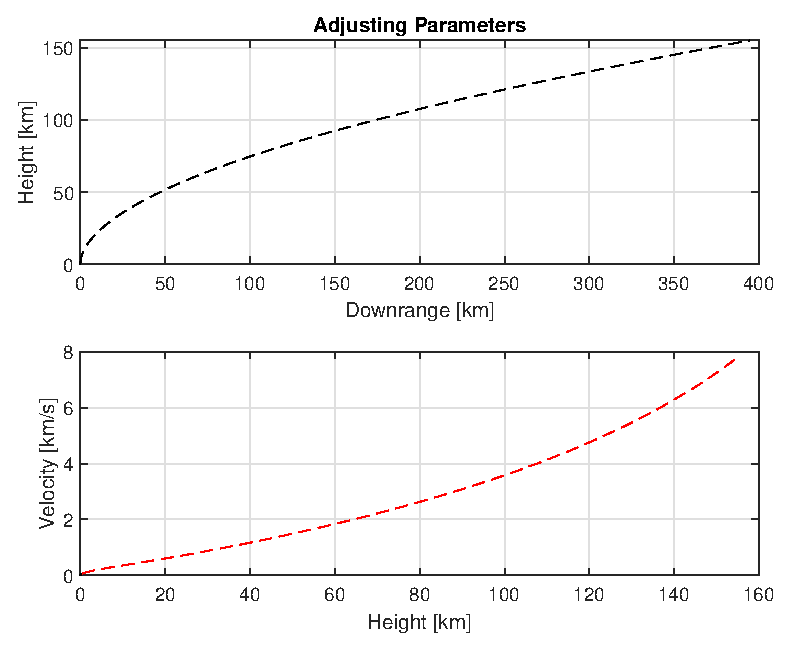
\includegraphics [width=4in]{RocketProblem_04.eps}


\subsection*{Rates function called by ODE45.}

\begin{verbatim}
function dydt = rocketMan(t, y)
    dydt = zeros(size(y));

    v = y(1);
    theta = y(2);
    x = y(3);
    h = y(4);

    if t < t_burn
       mass = mass_structure + mass_L + mass_P - m_dot * t;
       T = thrust;
    else
        T = 0;
        mass = mass_structure + mass_L;
    end

    g = -(mass * u) / (r_earth + h)^2;
    density = rho0 * exp(-h / hscale);
    drag = -0.5 * density * Cd * A * v^2;

    theta_dot = 0;
    v_dot = (T + drag + g) / mass;
    x_dot = 0;
    h_dot = v;

    dydt(1) = v_dot;
    dydt(2) = theta_dot;
    dydt(3) = x_dot;
    dydt(4) = h_dot;
end

function dydt = rocketMan2(t, y)
    dydt = zeros(size(y));

    v = y(1);
    theta = y(2);
    x = y(3);
    h = y(4);

    if t < t_burn
       mass = mass_structure + mass_L + mass_P - m_dot * t;
       T = thrust;
    else
        T = 0;
        mass = mass_structure + mass_L;
    end

    g = (mass * u) / (r_earth + h)^2;
    density = rho0 * exp(-h / hscale);
    drag = 0.5 * density * Cd * A * v^2;

    v_dot = (T - drag - g * cos(theta)) / mass;
    theta_dot = (u * sin(theta)) / (v * (r_earth + h)^2);
    x_dot = v*sin(theta);
    h_dot = v*cos(theta);

    dydt(1) = v_dot;
    dydt(2) = theta_dot;
    dydt(3) = x_dot;
    dydt(4) = h_dot;
end

function [value,isterminal,direction] = Begin_Pitch(~,y)
%Event funtion to stop integration when rocket reaches 500[m]
if y(4) < pitch
 value = 1; %Keep going
else %If not
 value = 0; %Then stop
end
isterminal = 1; %Terminate integration when condtion met
direction = 0; %Direction doesn't matter
end

function [value,isterminal,direction] = Crashed(~,y)
%Event funtion to stop integration when rocket reaches 500[m]
if y(4) > 0
 value = 1; %Keep going
else %If not
 value = 0; %Then stop
end
isterminal = 1; %Terminate integration when condtion met
direction = 0; %Direction doesn't matter
end
\end{verbatim}
\begin{verbatim}
end
\end{verbatim}



\end{document}
    
